% F(AI)^2R verification ladder as a finite-state machine.
% Source of truth: paper/figures/ladder-fsm.mmd (Mermaid stateDiagram).
% Build: rendered to paper/figures/ladder-fsm.pdf via mmdc; the
% Pages site renders the same .mmd client-side via mermaid.min.js so
% paper and site stay in lock-step. See paper/figures/ladder-fsm.figspec.md.
% This .tex shim is what % F(AI)^2R verification ladder as a finite-state machine.
% Source of truth: paper/figures/ladder-fsm.mmd (Mermaid stateDiagram).
% Build: rendered to paper/figures/ladder-fsm.pdf via mmdc; the
% Pages site renders the same .mmd client-side via mermaid.min.js so
% paper and site stay in lock-step. See paper/figures/ladder-fsm.figspec.md.
% This .tex shim is what % F(AI)^2R verification ladder as a finite-state machine.
% Source of truth: paper/figures/ladder-fsm.mmd (Mermaid stateDiagram).
% Build: rendered to paper/figures/ladder-fsm.pdf via mmdc; the
% Pages site renders the same .mmd client-side via mermaid.min.js so
% paper and site stay in lock-step. See paper/figures/ladder-fsm.figspec.md.
% This .tex shim is what % F(AI)^2R verification ladder as a finite-state machine.
% Source of truth: paper/figures/ladder-fsm.mmd (Mermaid stateDiagram).
% Build: rendered to paper/figures/ladder-fsm.pdf via mmdc; the
% Pages site renders the same .mmd client-side via mermaid.min.js so
% paper and site stay in lock-step. See paper/figures/ladder-fsm.figspec.md.
% This .tex shim is what \input{figures/ladder-fsm} from
% paper/sections/pattern.tex resolves to: it wraps the rendered PDF
% in a figure float with the manuscript caption.
\begin{figure}[!t]
\centering
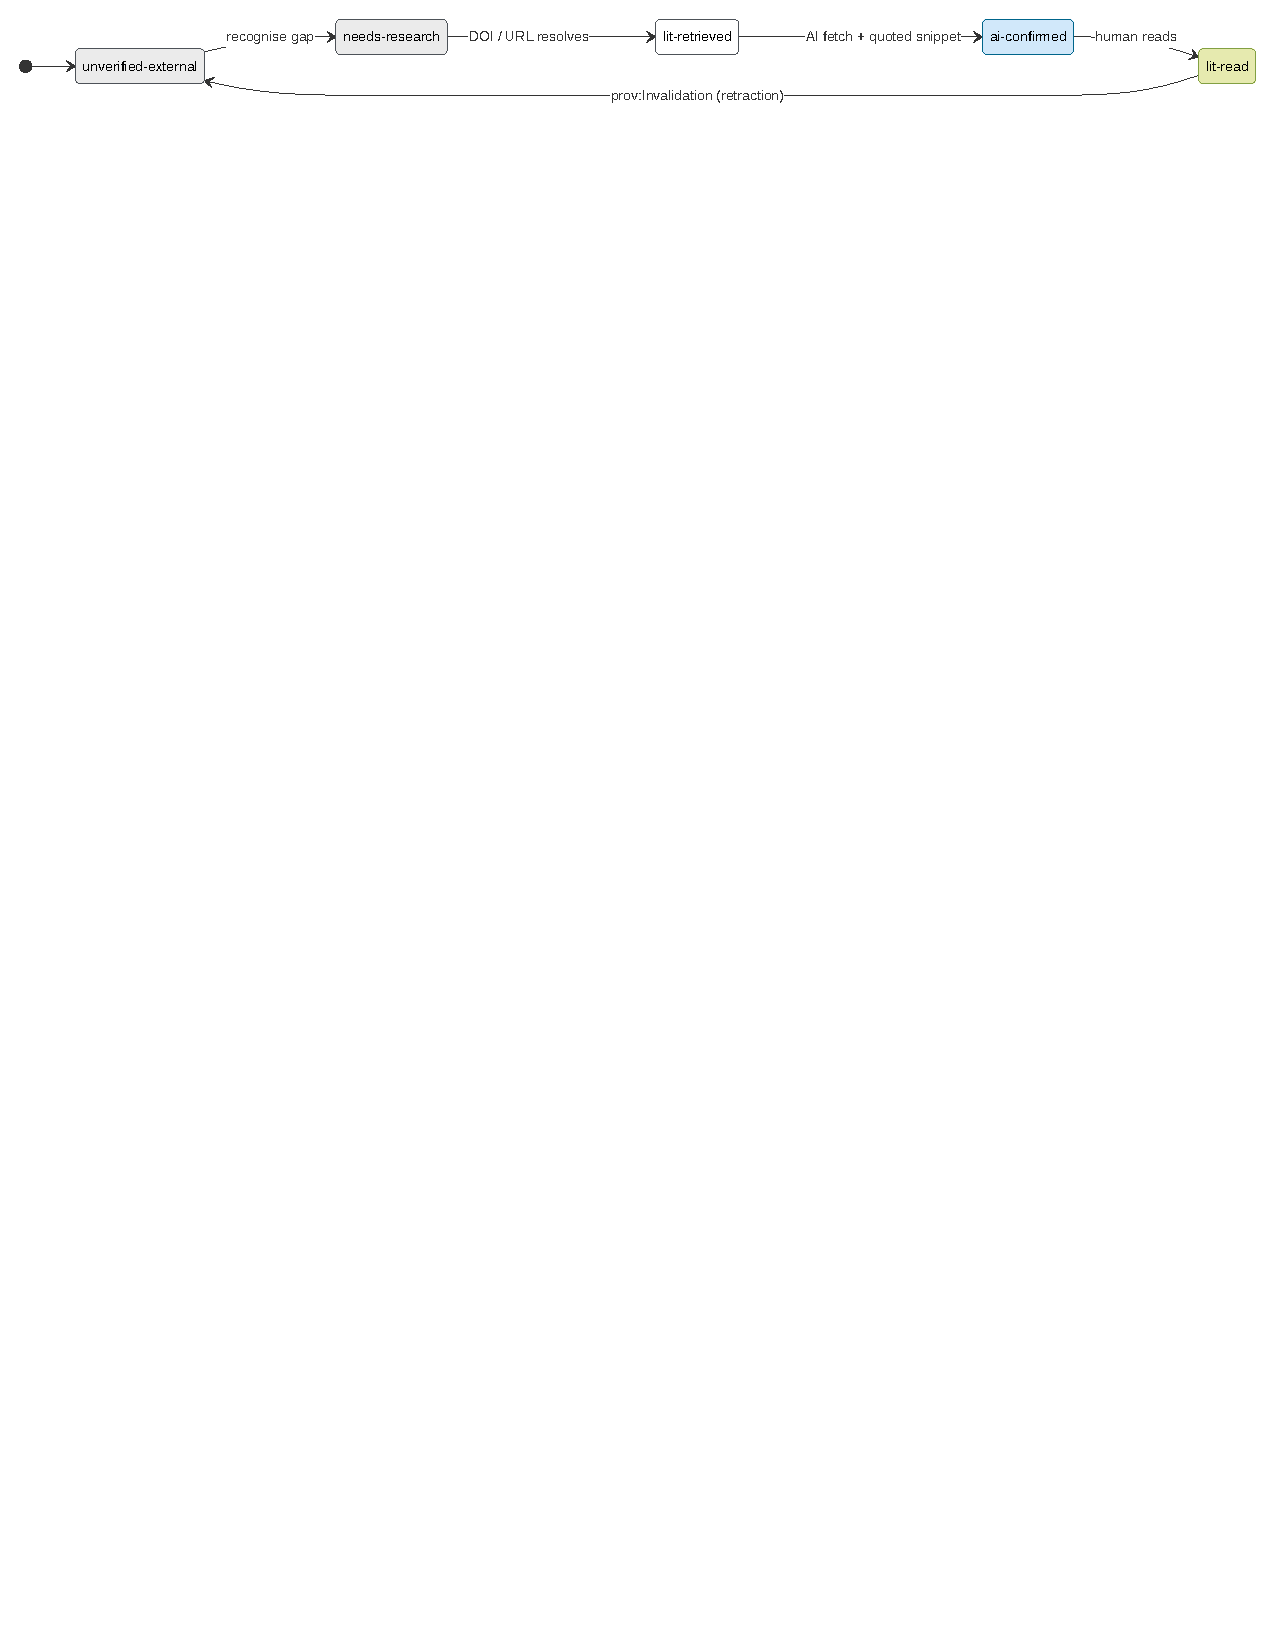
\includegraphics[width=0.92\linewidth]{figures/ladder-fsm.pdf}
\caption{The verification ladder as a finite-state machine. A
\texttt{fair2r:Claim} progresses left-to-right as evidence
accumulates; \textsc{ai-confirmed} is the ceiling an LLM agent can
deliver on its own (\S\ref{sec:ladder}). Retraction is the only
back-edge and is recorded as a \texttt{prov:Invalidation} activity
in \texttt{doc/provenance.ttl}, never as a deletion. A claim may be
\emph{invoked} at its current rung or below; load-bearing or
contested claims still require \textsc{lit-read}. Source: Mermaid
\texttt{stateDiagram-v2} at \texttt{paper/figures/ladder-fsm.mmd},
mirrored on the public site.}
\label{fig:ladder-fsm}
\end{figure}
 from
% paper/sections/pattern.tex resolves to: it wraps the rendered PDF
% in a figure float with the manuscript caption.
\begin{figure}[!t]
\centering
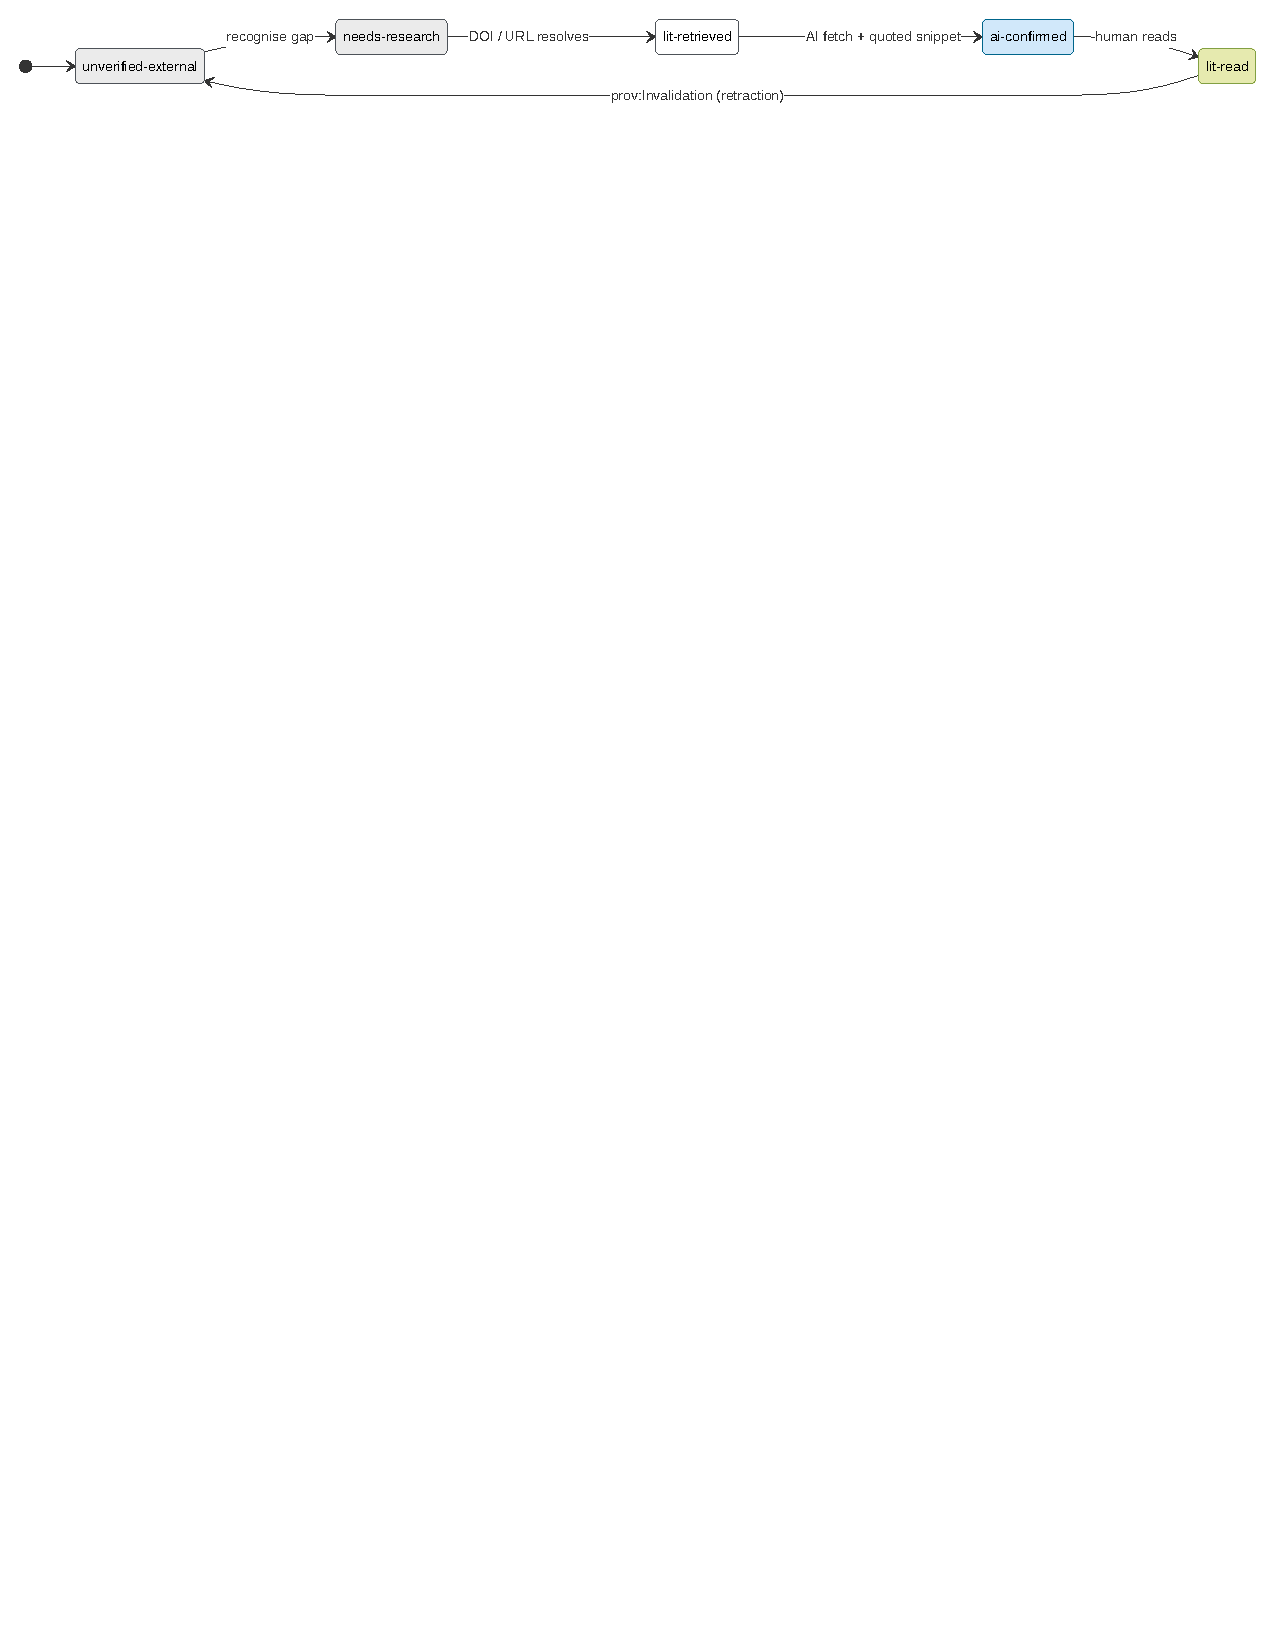
\includegraphics[width=0.92\linewidth]{figures/ladder-fsm.pdf}
\caption{The verification ladder as a finite-state machine. A
\texttt{fair2r:Claim} progresses left-to-right as evidence
accumulates; \textsc{ai-confirmed} is the ceiling an LLM agent can
deliver on its own (\S\ref{sec:ladder}). Retraction is the only
back-edge and is recorded as a \texttt{prov:Invalidation} activity
in \texttt{doc/provenance.ttl}, never as a deletion. A claim may be
\emph{invoked} at its current rung or below; load-bearing or
contested claims still require \textsc{lit-read}. Source: Mermaid
\texttt{stateDiagram-v2} at \texttt{paper/figures/ladder-fsm.mmd},
mirrored on the public site.}
\label{fig:ladder-fsm}
\end{figure}
 from
% paper/sections/pattern.tex resolves to: it wraps the rendered PDF
% in a figure float with the manuscript caption.
\begin{figure}[!t]
\centering
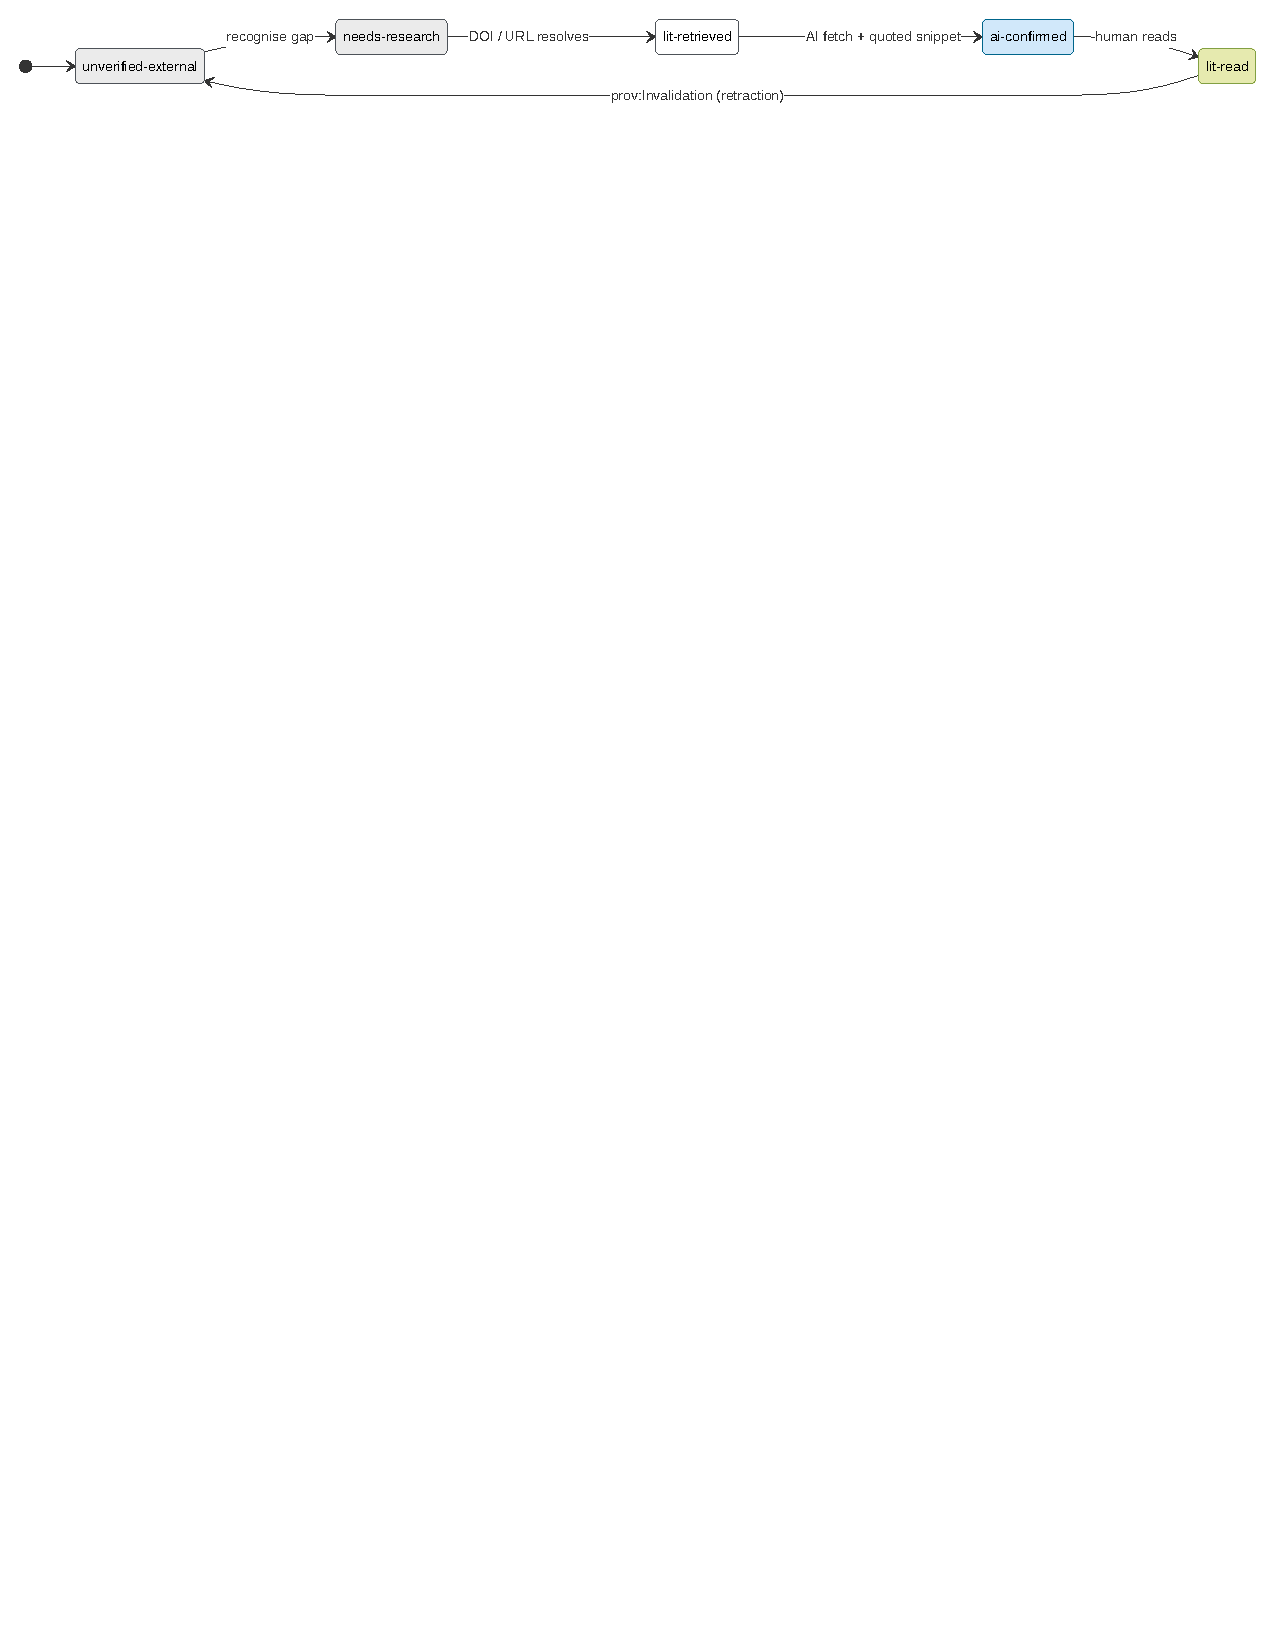
\includegraphics[width=0.92\linewidth]{figures/ladder-fsm.pdf}
\caption{The verification ladder as a finite-state machine. A
\texttt{fair2r:Claim} progresses left-to-right as evidence
accumulates; \textsc{ai-confirmed} is the ceiling an LLM agent can
deliver on its own (\S\ref{sec:ladder}). Retraction is the only
back-edge and is recorded as a \texttt{prov:Invalidation} activity
in \texttt{doc/provenance.ttl}, never as a deletion. A claim may be
\emph{invoked} at its current rung or below; load-bearing or
contested claims still require \textsc{lit-read}. Source: Mermaid
\texttt{stateDiagram-v2} at \texttt{paper/figures/ladder-fsm.mmd},
mirrored on the public site.}
\label{fig:ladder-fsm}
\end{figure}
 from
% paper/sections/pattern.tex resolves to: it wraps the rendered PDF
% in a figure float with the manuscript caption.
\begin{figure}[!t]
\centering
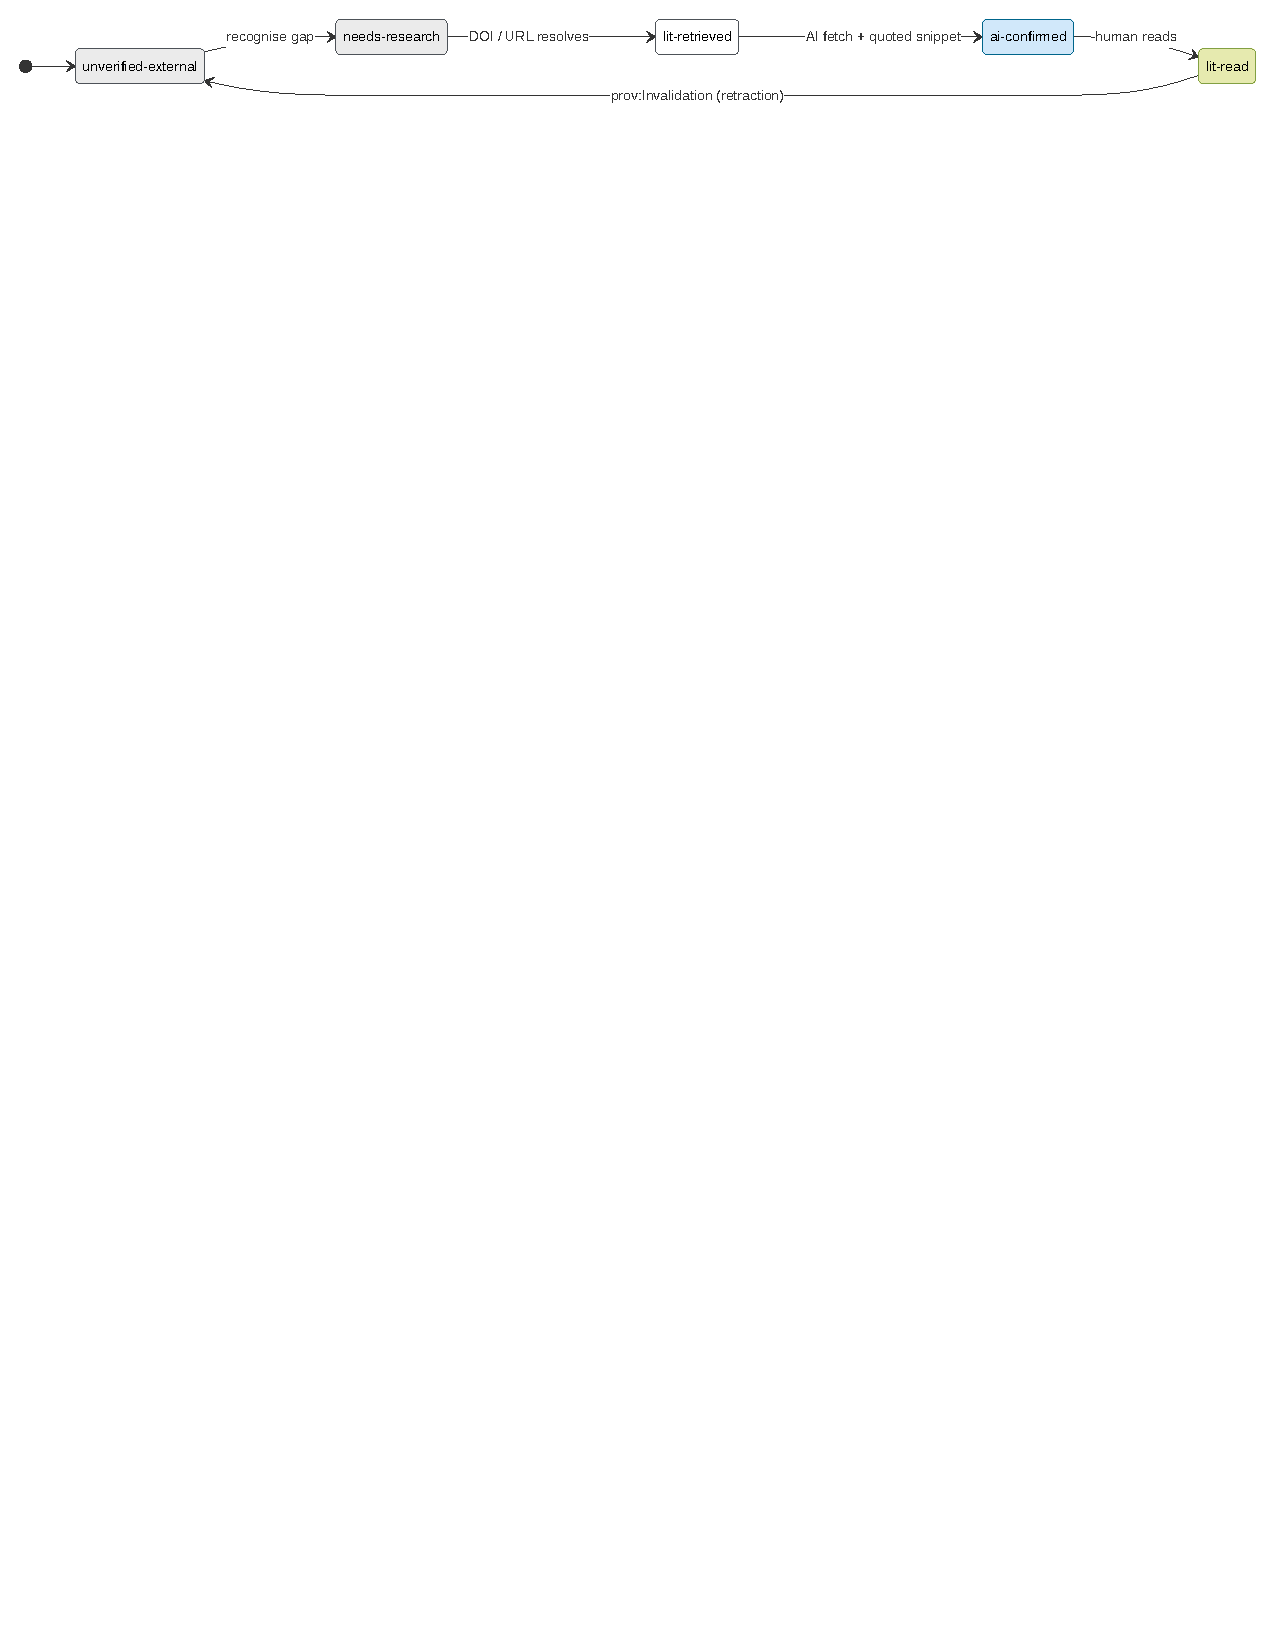
\includegraphics[width=0.92\linewidth]{figures/ladder-fsm.pdf}
\caption{The verification ladder as a finite-state machine. A
\texttt{fair2r:Claim} progresses left-to-right as evidence
accumulates; \textsc{ai-confirmed} is the ceiling an LLM agent can
deliver on its own (\S\ref{sec:ladder}). Retraction is the only
back-edge and is recorded as a \texttt{prov:Invalidation} activity
in \texttt{doc/provenance.ttl}, never as a deletion. A claim may be
\emph{invoked} at its current rung or below; load-bearing or
contested claims still require \textsc{lit-read}. Source: Mermaid
\texttt{stateDiagram-v2} at \texttt{paper/figures/ladder-fsm.mmd},
mirrored on the public site.}
\label{fig:ladder-fsm}
\end{figure}
